\documentclass[12pt,english]{article}
\usepackage{geometry}
\usepackage{float}
\usepackage{caption}
\geometry{verbose,tmargin=3cm,bmargin=3cm,lmargin=3cm,rmargin=3cm}
\usepackage{amsmath}
\usepackage{amssymb}
\usepackage{amsthm}
\usepackage{adjustbox}
\usepackage{hyperref}
\usepackage{graphicx}
\usepackage{setspace}
\usepackage{changepage}
\onehalfspacing
\usepackage{babel}
\newcommand{\expec}{\ensuremath{\mathbb E}}
\begin{document}
\begin{center}
{\Large{}Section 4: Access to credit} \\
{\large{}Banerjee and Duflo (2014)}
\par\end{center}{\Large \par}

\begin{center}
EEP 152
\par\end{center}

\begin{center}
September 21, 2016
\par\end{center}

\begin{itemize}
	\setlength\itemsep{-0.5em}
	\item DID (10 min)
	\item Banerjee and Duflo (2014) and discussion (40 min)
\end{itemize}
A copy of a public version of the paper is available on the section Github at \href{github.com/johnloeser/eep152}{github.com/johnloeser/eep152} in the ``section4'' folder.\footnote{The published version clarifies a few things relative to this version. If you'd like to download that, you can get access to the published version if you're connected to AirBears2.} If you missed the first three sections, it would be useful to briefly go through the section syllabus, also available on the section Github.

\section{Difference in differences (DID)}

As we discussed last week, we're often interested in estimating the effect of some treatment (for example, a cash grant) on some economic outcome (for example, profits). Ideally, to accurately estimate the effect of the treatment on the outcome, we would like to randomly assign access to the treatment across households or locations. In some cases, this may be infeasible or unethical. How can we estimate the effect of the treatment in those cases?

For example, let's consider the question ``What is the effect of access to credit on firm revenue?'' If we randomly assigned access to credit across firms, we can use the control group (the group that randomly did not receive access to credit) as the counterfactual for the treatment group (the group that randomly did receive access to credit). In other words, we assume that the treatment group would have had the same outcomes as the control group (on average) if they hadn't randomly received access to credit.

Now instead, let's suppose that we can't randomly assign access to credit. Instead, we just look at firms that are borrowing money (who we'll still call treatment firms), and firms that aren't borrowing money (who we'll still call control firms). The problem is that it's probably not a reasonable assumption that treatment firms would have had the same outcomes as control firms if they did not have access to credit --  there might be a large number of reasons that treatment firms get access to credit and control firms do not that also drive differences in revenue between the two groups.

However, what if we can observe the firms that borrowed money before they started borrowing money? We still have the problem that firms that are granted access to credit are likely different from firms that are not granted access to credit. However, instead of assuming that the control firms' revenues are a valid counterfactual for the treatment firms' revenues, we can instead assume that the control firms' \textit{changes} in revenue are a valid counterfactual for the treatment firms' \textit{changes} in revenue.

\begin{center}
	\begin{adjustbox}{
			max width=0.65\textwidth,
		}
		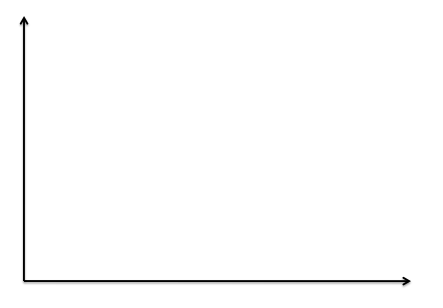
\includegraphics{axes.png}
	\end{adjustbox}
\end{center}

This may not always be a reasonable assumption. However, there are often a few ways we can test this. First, we can use other periods that occurred before treatment firms received access to credit. In those periods, even if the revenues of treatment and control firms are still different, if the changes in revenue of the treatment and control firms were the same, this suggests that those trends would have continued to be the same even if the treatment firms had not received access to credit (this is known as the ``parallel trends'' test).

\begin{center}
	\begin{adjustbox}{
			max width=0.65\textwidth,
		}
		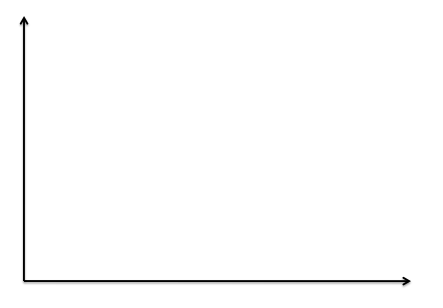
\includegraphics{axes.png}
	\end{adjustbox}
\end{center}

Second, we can try to use our understanding of the treatment (in this case, access to credit) to make predictions about which outcomes should and should not be affected. For example, in response to an increase in access to credit, we should expect firms to make investments in capital or labor, but we might not expect firms to have increases in productivity. If treatment firms appear to have larger increases in productivity without increases in capital (both relative to the control firms), this suggests we are not estimating the true effect of access to credit.

\section{Banerjee and Duflo (2014)}

In class, we discussed estimating the effect of expanded access to formal banking on rural villages in India. By competing with moneylenders (who charge high interest rates), we might expect this to have an effect on the poverty of households by providing access to cheaper credit.

In ``Do firms want to borrow more?'', Banerjee and Duflo (BD hereafter) make the point that there are two possible explanations of the reduction in poverty observed. First, moneylenders charge higher interest rates than banks, so access to banks reduces the interest rates you pay. As a result, the households become richer. Second, households may be credit constrained -- in other words, even at the high interest rates they pay, households would like to borrow more money. Banks may be able to alleviate this constraint, while moneylenders may not (if, for example, moneylenders have a small amount of working capital compared to banks). However, instead of studying rural households, BD study medium and large businesses.

BD are not able to randomize access to credit for these banks -- doing so would be extremely expensive, and banks would not agree to it. Instead, they make use of two policy changes to regulations mandating banks lend 40\% of credit to ``priority sector'' firms. Historically, the definition of this sector was firms operating in a few industries with investments below about \$100,000. However, in January 1998, this cutoff was raised to about \$500,000, and in January 2000 the cutoff was again lowered to about \$200,000. In their terminology, ``small'' firms always were priority sector, ``medium'' and ``biggest'' firms were included in the priority sector in 1998 and 1999, and ``biggest'' firms were excluded from the priority sector after 2000.

\begin{center}
	\begin{adjustbox}{
			max width=0.65\textwidth,
		}
		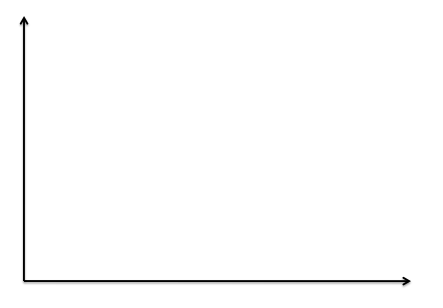
\includegraphics{axes.png}
	\end{adjustbox}
\end{center}

We'll focus on the how to estimate the effects of access to credit on borrowing and firm revenue for the biggest firms using the policy change. In particular, we can see that the biggest firms experienced two shocks -- first, they had an increase in access to credit in January 1998, and second, they had a decrease in access to credit in January 2000. Let's use $Y$ to denote firm revenue, and $\ell$ to denote firm borrowing. How can we estimate the effect of each of these shocks on $Y$ and $\ell$?

\begin{figure}[H]
	\begin{minipage}{.5\textwidth}
		\centering
		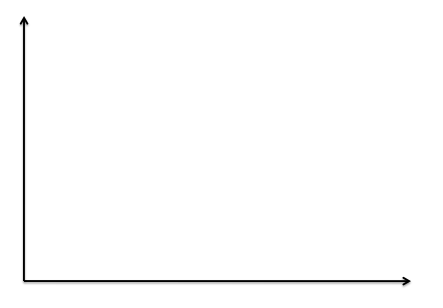
\includegraphics[width = \textwidth]{axes.png}
	\end{minipage}
	\begin{minipage}{.5\textwidth}
		\centering
		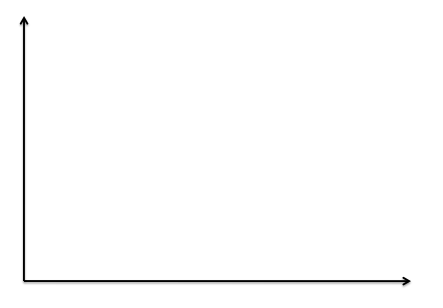
\includegraphics[width = \textwidth]{axes.png}
	\end{minipage}
\end{figure}

We can see that the small firms might provide a valid control group for the biggest firms. Let $\beta_{Y1}$ and $\beta_{Y2}$ denote the effect of the first policy change and the second policy change on firm revenues. Then, we can use DID to calculate

$$ \beta_{Y1} = \left( \overline{Y_{\text{biggest}, 1999}} - \overline{Y_{\text{small}, 1999}} \right) - \left( \overline{Y_{\text{biggest}, 1997}} - \overline{Y_{\text{small}, 1997}} \right) $$
$$ \beta_{Y2} = \left( \overline{Y_{\text{biggest}, 2001}} - \overline{Y_{\text{small}, 2001}} \right) - \left( \overline{Y_{\text{biggest}, 1999}} - \overline{Y_{\text{small}, 1999}} \right) $$

In particular, for a selected set of firms\footnote{This is restricting to the sample of firms whose credit limits change. I'm not really sure why this is done in the paper, but not all of these effects are available for the full sample.}, BD estimate $\beta_{\ell1} = 35\%$, $\beta_{\ell2} = -48\%$, $\beta_{Y1} = 24\%$, and $\beta_{Y2} = -42\%$. The reform significantly increased the credit available to and sales of the ``biggest'' firms, and the second reform significantly decreased the credit available to and sales of these firms.

Should we believe these results? First, we would like to implement a parallel trends test that we mentioned earlier. This is not possible for the biggest firms (because BD do not have data before 1997), but an alternative version of this test is available for the medium firms -- in particular, we expect the medium firms, relative to the small firms, to see increases in their borrowing and sales following the first reform, but not following the second firm. BD test this, and they find this to be the case.

Second, we can use a model to put restrictions on $\beta_{\ell1}$, $\beta_{\ell2}$, $\beta_{Y1}$, and $\beta_{Y2}$. There are two sets of restrictions BD use. 

First, given the description of the policy, we should expect these reforms to cancel each other out. In particular, $\beta_{\ell1} + \beta_{\ell2} = 0$ and $\beta_{Y1} + \beta_{Y2} = 0$. Although these aren't exactly 0 when we calculate them, they are not statistically significantly different from 0 (although it's impossible for you to know this since I didn't provide the standard errors), so BD's estimated effects pass this test.

Second, both the first and second reform allow us to estimate the effect of borrowing on sales for these firms. In particular, assuming the reform only affects sales by increasing firm borrowing, we can look at the change in sales the firms experience because of the reform, and divide by the change in borrowing because of the reform.
$$ \frac{\%dY}{\%d\ell} = \frac{\beta_{Y1}}{\beta_{\ell1}} = \frac{\beta_{Y2}}{\beta_{\ell2}} $$
The two estimates of $\frac{\%dY}{\%d\ell}$ should be equal, since we do not expect the reform to affect firm productivity. This is what BD find - both reforms yield estimates of 70\% to 80\% for $\frac{\%dY}{\%d\ell}$.

Finally, interpreting this number is more difficult. What does the percentage increase in income because of a 1\% increase in borrowing mean? Instead, to get back to the MPK that we discussed earlier, they use the reform to estimate the effect of a \$1 increase in borrowing on firm profits, and estimate annul $\text{MPK} \approx 0.9$. As we've now seen with microenterprises in Ghana and Sri Lanka, entrepreneurs in Nigeria, and now medium to large firms in India, high MPK and limited access to credit appears characteristic of firms in poor countries. In India, however, the case seems more mysterious -- these are large firms that have significant collateral available, and yet this study provides evidence that these firms are credit constrained. Why aren't these firms able to borrow more?

\end{document}